

\begin{figure}[ht!]
  \begin{center}
    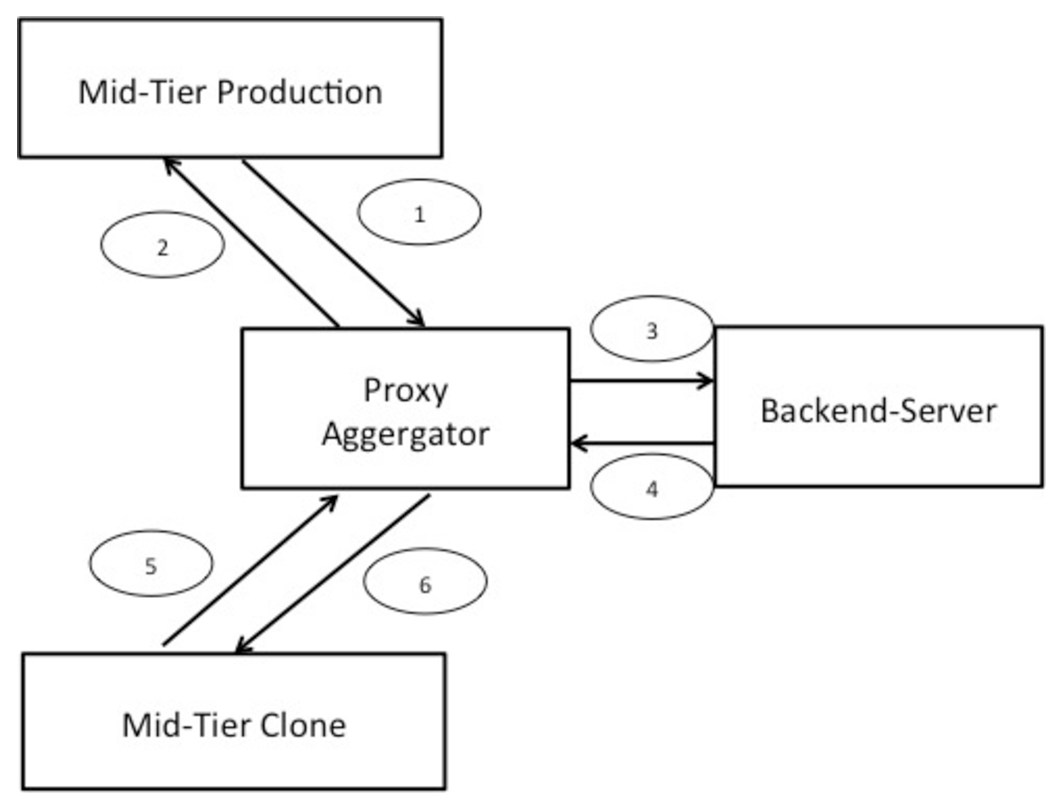
\includegraphics[width=0.4\textwidth]{figs/aggregator.eps}
    \caption{Description of the Network Aggregator}
    \label{fig:aggregator}
  \end{center}
\end{figure}

\subsection{Proxy Network Aggregator \& Replay }
\label{sec:proxyAggregator}

The proxy described in section \ref{sec:proxyDuplicator} is used to communicate to downstream tiers and replicate traffic being sent to production tiers in the debug containers.
This manages incoming ``requests'' to the target container, however the same mechanism cannot be directly applied for isolating responses sent to the target container. 
Imagine if you are trying to debug a mid-tier application container, the proxy network duplicator will replicate all incoming traffic from the client to both debug and the production container. 
Both the debug container and the production, will then try to communicate further to the back-end containers.
This could mean duplicate queries(duplicate delete to mysql for instance) to the backend servers, and could hence lead to an inconsistent state.
The ``proxy aggregator'' module sandboxes the impact any requests from a duplicate debug container, and manages responses to the debug container, by replaying the proxy containers responses.

As shown in the fig \ref{fig:aggregator}, when an incoming request comes to the aggregator, it first checks if the connection is from the production container or debug container. 
In case of the production container, the aggregator forwards the connection to the backend (link 3), responses from the backend are sent to the aggregator (link 4), and then forwarded to the production container (link 2) and simultaneously saved in an internal queue.
The aggregator creates an in-memory persistent inter-process FIFO queue for each connection where the responses for each of these connections are stored.
When the corresponding connection from the duplicate debug container connects to the proxy (link 5); all packets being sent are quietly dropped, responses are sent from the queue and sends it to the debug container(link 6).
Since we assume that the production and the debug container are in the same state, and are sending the same requests, sending the corresponding responses from the FIFO stack instead of the backend ensures: (a) all communications to and from the debug container are isolated from the rest of the network, (b) the debug container gets a logical response for all it's outgoing requests, thereby behaving logically correctly.

In this design we assume that the order of incoming connections remains largely the same.
We use a fuzzy checking mechansim using the hash value of the data being sent to correlate the connections. 
In case a connection is out of order or cannot be correlated, we allow the connection to time out and send a TCP\_FIN.

